\documentclass[12pt]{article}
%\usepackage[utf8]{inputenc}
%\documentclass[UTF8]{ctexart}
%\usepackage[UTF8, heading = false, scheme = plain]{ctex}
\usepackage{geometry}
%geometry{a4paper,scale=0.9}
\geometry{a4paper,left=1cm,right=1cm,top=1cm,bottom=2cm}
\usepackage{amsfonts}
\usepackage{color}
\usepackage{url}
%\usepackage{biblatex}
\usepackage{amsmath}
\usepackage{amssymb}
\usepackage{latexsym}
\usepackage[linesnumbered,ruled,lined]{algorithm2e}
\usepackage{pythonhighlight}
\usepackage{cite}
%\addbibresource{ref.bib}
%\bibliography{ref.bib}
\usepackage{caption}
\usepackage{graphicx, subfig}
\usepackage{float}
%\usepackage[fontset=ubuntu]{ctex}
%\usepackage{fontspec}
\usepackage{xeCJK}
%\usepackage[colorlinks,
%anchorcolor=black,
%citecolor=black]{hyperref}
%\setmainfont{SimSun}
\usepackage[section]{placeins}
\usepackage{enumitem}
\usepackage{framed}
\usepackage[framemethod=TikZ]{mdframed}
\usepackage{indentfirst}
\usepackage{setspace}%使用间距宏包
\linespread{1.5}

\title{Yolo 系列解读\cite{Yolo_From_V1_To_V5_1}}
\author{leolinuxer}
%\date{June 2020}

\begin{document}
%\setlength{\parindent}{0pt}
\maketitle
\tableofcontents

\section{相关背景}
\subsection{图像分类和检测}
在进入目标检测任务之前首先得学会图像分类任务,这个任务的特点是输入一张图片,输出是它的类别。
\begin{itemize}
\setlength{\itemsep}{0pt}
\setlength{\parsep}{0pt}
\setlength{\parskip}{0pt}
    \item 对于输入图片,我们一般用一个矩阵表示;
    \item 对于输出结果,我们一般用一个one-hot vector表示:$[0, 0, 1, 0, 0, 0]$,哪一维是1,就代表图片属于哪一类。
\end{itemize}

检测器和分类器的区别:
\begin{itemize}
\setlength{\itemsep}{0pt}
\setlength{\parsep}{0pt}
\setlength{\parskip}{0pt}
    \item 他们的输入都是image;
    \item 分类器的输出是一个one-hot vector,而检测器的输出是一个框(Bounding Box)。
\end{itemize}

\subsection{检测器结果的表示方法}
在一个图片里面表示一个框,有很多种方法,比如:
\begin{itemize}
\setlength{\itemsep}{0pt}
\setlength{\parsep}{0pt}
\setlength{\parskip}{0pt}
    \item x,y,w,h;
    \item p1,p2,p3,p4(4个点坐标);
    \item cx,cy,w,h(cx,cy为中心点坐标);
    \item x,y,w,h,angle(还有的目标是有角度的,这时叫做Rotated Bounding Box);
    \item ……
\end{itemize}

不管用什么形式去表达这个Bounding Box,检测器模型输出的结果一定是一个vector,那这个vector和分类模型输出的vector本质上有什么区别吗?答案是:没有,都是向量而已。只是分类模型输出是one-shot向量,检测模型输出是我们标注的结果。

\subsection{基于分类模型的检测任务}
所以你应该会发现,检测的方法呼之欲出了。那分类模型可以用来做检测吗?当然可以,这时,你可以把检测的任务当做是遍历性的分类任务。

遍历的方法就是用不同尺寸的矩形框,去遍历图像,执行分类任务,专业术语叫做:滑动窗口分类方法。这种方法的精度和遍历是否彻底密切相关,遍历得越精确,检测器的精度就越高。所以这也就带来一个问题就是:检测的耗时非常大。

\section{Yolo 系列的思想}
\subsection{Yolo V0}
YOLO的作者当时是这么想的:你分类器输出一个one-hot vector,那我把它换成(x,y,w,h,c),c表示confidence置信度,把问题转化成一个回归问题,直接回归出Bounding Box的位置不就好了吗?\textbf{本质上都是矩阵映射到向量,只是代表的意义不一样而已}。

那如何组织训练呢?找到足够的训练集,把 label 设置为 $(1, x^*, y^*, w^*, h^*)$,这里 $x^*$ 代表真值。有了数据和label,就完成了设计。

我们会发现,这种方法比刚才的滑动窗口分类方法简单太多了。这一版的思路我把它叫做YOLO v0,因为它是You Only Look Once最简单的版本。

\subsection{Yolo V1}
但是 YOLO v0只能输出一个目标,如何识别个多目标呢?

你可能会回答:我输出N个向量不就行了吗?但具体输出多少个合适呢?这个N又该如何调整呢?答案是:为了保证所有目标都被检测到,我们应该输出尽量多的目标。

比如将图片设置为16个区域,每个区域用1个(c,x,y,w,h)去负责,就可以一次输出16个框,每个框是1个(c,x,y,w,h),如图所示:
\begin{figure}[H]
    \centering
    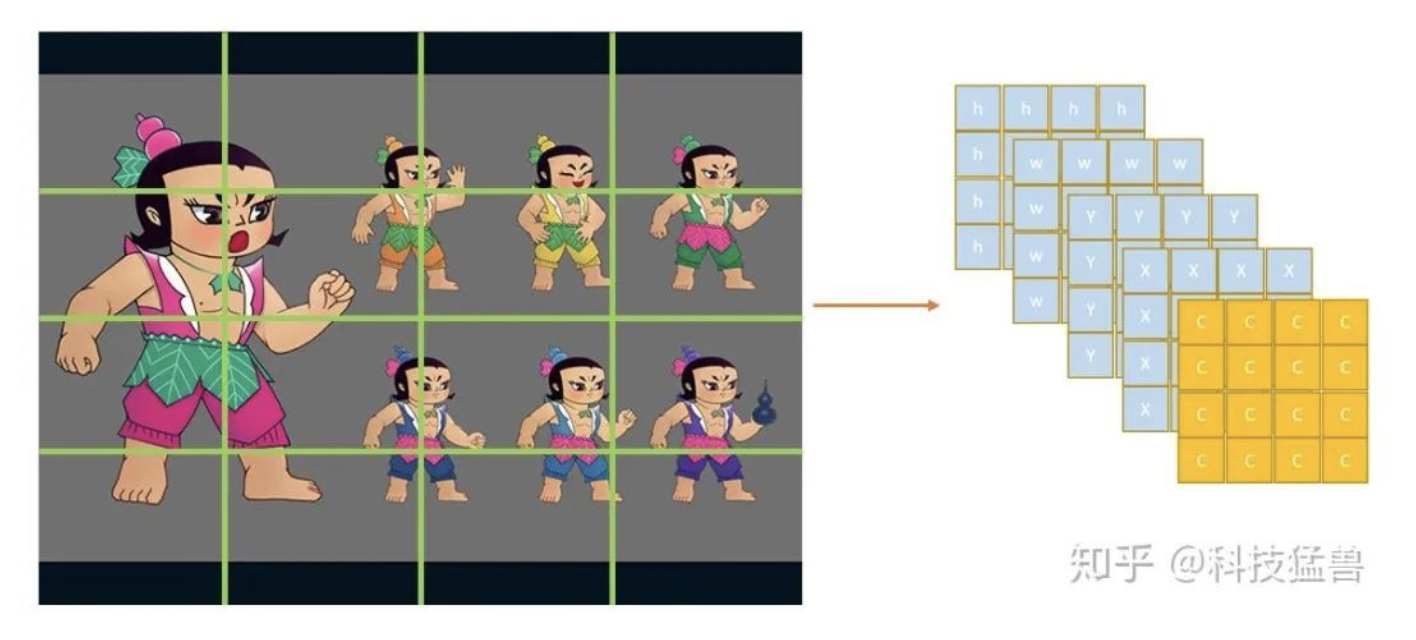
\includegraphics[width=.6\textwidth]{fig/Yolo_Series_1.png}
\end{figure}

为什么这样子更优?因为conv操作是位置强相关的,就是原来的目标在哪里,你conv之后的feature map上还在哪里,所以图片划分为16个区域,结果也应该分布在16个区域上,所以我们的结果(Tensor)的维度size是:(5,4,4)。

那现在你可能会问:c的真值该怎么设置呢?

答:看葫芦娃的大娃,他的脸跨了4个区域(grid),但只能某一个grid的c=1,其他的c=0。那么该让哪一个grid的c=1呢?就看他的脸的中心落在了哪个grid里面。根据这一原则,c的真值为下图7所示:
\begin{figure}[H]
    \centering
    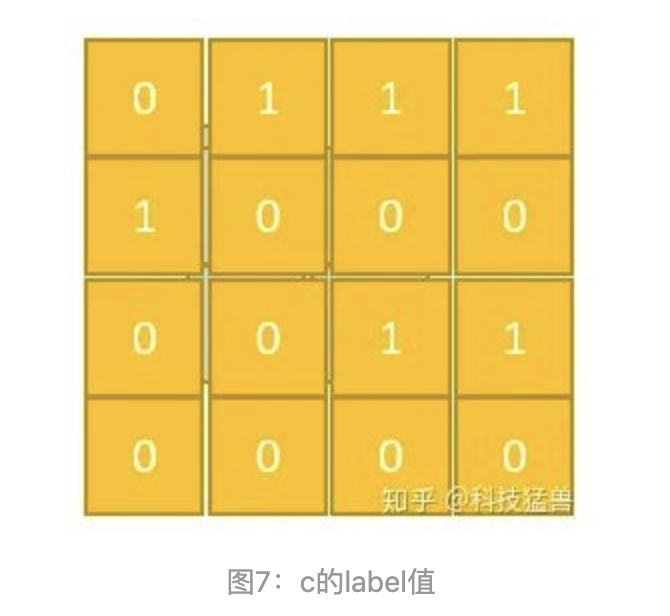
\includegraphics[width=.4\textwidth]{fig/Yolo_Series_2.png}
\end{figure}

但是你发现7个葫芦娃只有6个1,原因是某一个grid里面有2个目标,确实如此,第三行第三列的grid既有水娃又有隐身娃。这种一个区域有多个目标的情况我们目前没法解决,因为我们的模型现在能力就这么大,只能在一个区域中检测出一个目标。改进方法后面讨论

总之现在我们设计出了模型的输出结果,那距离完成模型的设计还差一个损失函数,那Loss咋设计呢?看下面的伪代码:
\begin{python}
loss = 0
for img in img_all:
   for i in range(3):
      for j in range(4):
         loss_ij = lamda_1*(c_pred-c_label)**2 + c_label*(x_pred-x_label)**2 +\
                     c_label*(y_pred-y_label)**2 + c_label*(w_pred-w_label)**2 + \
                     c_label*(h_pred-h_label)**2
         loss += loss_ij
loss.backward()
\end{python}

遍历所有图片,遍历所有位置,计算loss。

现在回到刚才的问题:模型现在能力就这么大,只能在一个区域中检测出一个目标,如何改进?答案是:刚才区域是 4*4,可以变成40*40,将区域变得更密集,就可以缓解多目标的问题,但是无法从根本上解决。

另一个问题,按上面的设计你检测得到了16个框,可是图片上只有7个葫芦娃的脸,怎么从16个结果中筛选出7个我们要的呢?

方法1:聚类。聚成7类,在这7个类中,选择confidence最大的框。听起来挺好。问题是:2个目标本身比较近聚成了1个类怎么办?如果不知道到底有几个目标呢?为何聚成7类?不是3类?

法2:NMS(非极大值抑制)。2个框重合度很高,大概率是一个目标,那就只取一个框。重合度的计算方法:交并比IoU=两个框的交集面积/两个框的并集面积。

具体算法:
\begin{figure}[H]
    \centering
    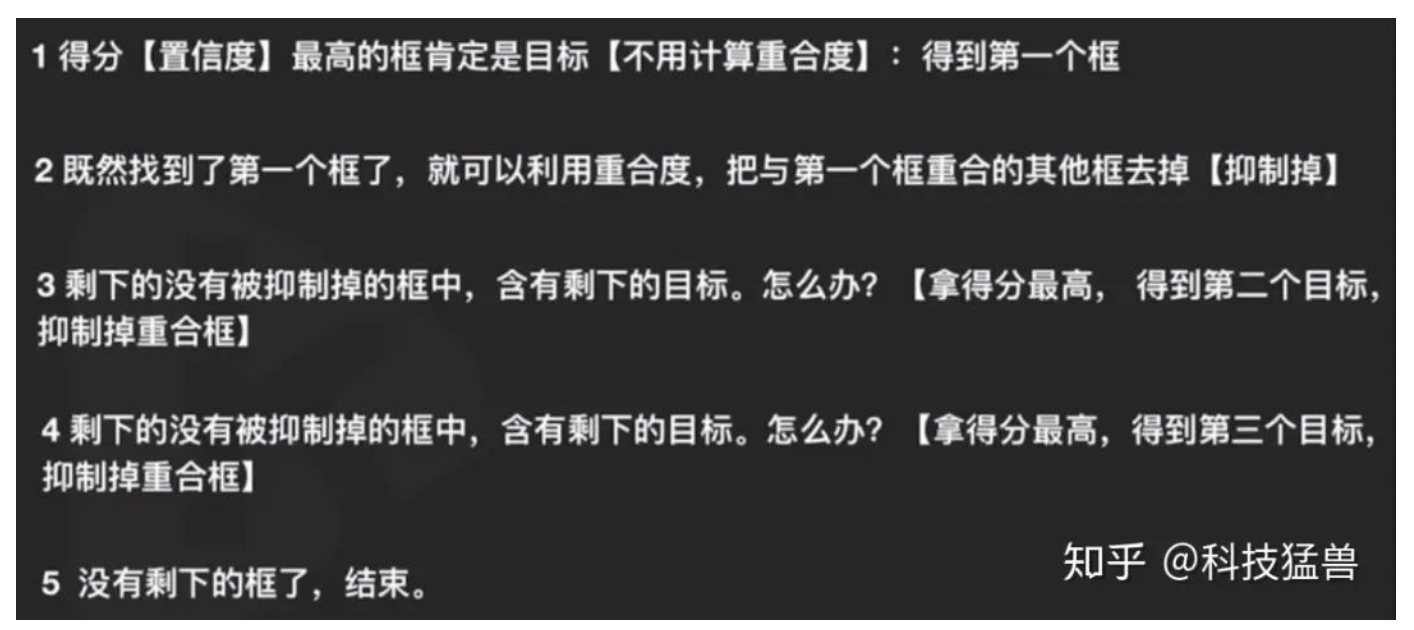
\includegraphics[width=1\textwidth]{fig/Yolo_Series_3.png}
\end{figure}

法1的bug:2个目标本身比较近怎么办?依然没有解决。

如果不知道到底有几个目标呢?NMS自动解决了这个问题。

面试的时候会问这样一个问题:NMS的适用情况是什么?

答:1图多目标检测时用NMS。

到现在为止我们终于解决了第4节开始提出的多个目标的问题,现在又有了新的需求:

需求2:多类的目标怎么办呢?2个类,one-hot就是[0,1],[1,0]这样子,



%\printbibliography
\bibliography{../ref}
\bibliographystyle{IEEEtran}
\end{document}
